% ============================================================
%  يُترجَم بـ XeLaTeX  (في Overleaf: Menu → Compiler → XeLaTeX)
%  الخط: Amiri (متوفر في Overleaf، أو حمّله من github.com/aliftype/amiri)
% ============================================================
\documentclass[12pt,a4paper]{article}
\usepackage[a4paper,margin=1.7cm,top=2.3cm,bottom=2.9cm,headheight=15pt,footskip=1.5cm]{geometry}
\usepackage{amsmath,amssymb}
\usepackage{icomma}
\usepackage[english,bidi=default,layout=lists]{babel}
\babelprovide[import,main]{arabic}
\babelfont{rm}[Scale=1.08]{Amiri}
\babelfont{sf}[Scale=1.08]{Amiri}
\usepackage[most]{tcolorbox}
\usepackage{tikz}
\usetikzlibrary{arrows.meta,calc,shadings}
\usepackage{array}
\usepackage{colortbl}
\usepackage{fancyhdr}
\usepackage{titlesec}
\usepackage{enumitem}
\usepackage{collcell}
\usepackage{needspace}
\usepackage{etoolbox}
% أعمدة جداول تُكتب خلاياها بالعربية في الاتجاه الصحيح
\newcolumntype{C}{>{\collectcell\ar}c<{\endcollectcell}}
% تجنب عنوان يتيم في أسفل الصفحة
\pretocmd{\section}{\Needspace{15\baselineskip}}{}{}
\pretocmd{\subsection}{\Needspace{11\baselineskip}}{}{}

% ---------- الألوان ----------
\definecolor{cDef}{HTML}{1F4E9C}
\definecolor{cThm}{HTML}{B3261E}
\definecolor{cRem}{HTML}{2E7D32}
\definecolor{cEx}{HTML}{C76B00}
\definecolor{cMeth}{HTML}{6A1B9A}
\definecolor{cSol}{HTML}{00695C}
\definecolor{cSec}{HTML}{1F3A68}

% ---------- العناوين ----------
\titleformat{\section}{\Large\bfseries\color{cSec}}{\thesection.}{0.6em}{}[{\color{cSec!60}\titlerule[1pt]}]
\titleformat{\subsection}{\large\bfseries\color{cThm!85!black}}{\thesubsection.}{0.5em}{}
\titlespacing*{\section}{0pt}{14pt}{8pt}
\titlespacing*{\subsection}{0pt}{10pt}{5pt}
\setlength{\parindent}{0pt}
\setlength{\parskip}{4pt}
\setlist{itemsep=2pt,topsep=3pt}

% ---------- الصناديق (تُرسم في سياق LTR ويُكتب محتواها بالعربية) ----------
\newtcolorbox{arbox}[3][]{enhanced,
  colback=#2!5,colframe=#2!80!black,arc=2mm,boxrule=0.8pt,
  left=6pt,right=6pt,top=8pt,bottom=5pt,
  fonttitle=\bfseries,coltitle=white,
  title={\foreignlanguage{arabic}{#3}},
  attach boxed title to top right={xshift=-5mm,yshift=-3mm},
  boxed title style={colback=#2!80!black,arc=1.5mm,boxrule=0pt},
  before upper={\selectlanguage{arabic}},
  before skip=8pt,after skip=8pt,breakable,#1}
\newenvironment{BOX}[2]{\begin{otherlanguage}{english}\begin{arbox}{#1}{#2}}{\end{arbox}\end{otherlanguage}}
\newenvironment{tarif}[1][تعريف]{\begin{BOX}{cDef}{#1}}{\end{BOX}}
\newenvironment{khassia}[1][خاصية]{\begin{BOX}{cThm}{#1}}{\end{BOX}}
\newenvironment{molahada}[1][ملاحظة]{\begin{BOX}{cRem}{#1}}{\end{BOX}}
\newenvironment{mithal}[1][مثال]{\begin{BOX}{cEx}{#1}}{\end{BOX}}
\newenvironment{tariqa}[1][طريقة]{\begin{BOX}{cMeth}{#1}}{\end{BOX}}

% ---------- التمارين والحلول ----------
\newcounter{exo}
\newenvironment{tamrin}[1]{\stepcounter{exo}\begin{BOX}{cSec}{التمرين \theexo: #1}}{\end{BOX}}
\newenvironment{hal}{\Needspace{12\baselineskip}\begin{otherlanguage}{english}\begin{arbox}[breakable]{cSol}{حل التمرين \theexo}}{\end{arbox}\end{otherlanguage}}

% رسومات TikZ تُوضع في سياق LTR
\newenvironment{LTR}{\begin{otherlanguage}{english}}{\end{otherlanguage}}
\newcommand{\ar}[1]{\foreignlanguage{arabic}{#1}}

% ---------- رموز ----------
% نقاط الحذف داخل الرياضيات (\dots يسبب خللاً في الاتجاه مع babel)
\renewcommand{\dots}{\mathinner{\ldotp\ldotp\ldotp}}
\renewcommand{\ldots}{\mathinner{\ldotp\ldotp\ldotp}}
\renewcommand{\cdots}{\mathinner{\cdotp\cdotp\cdotp}}
\newcommand{\N}{\mathbb{N}}
\newcommand{\Z}{\mathbb{Z}}
\newcommand{\D}{\mathbb{D}}
\newcommand{\Q}{\mathbb{Q}}
\newcommand{\R}{\mathbb{R}}
\newcommand{\pgcd}{\operatorname{PGCD}}
\newcommand{\ppcm}{\operatorname{PPCM}}

% ---------- تمثيل مجال على مستقيم عددي ----------
% \NLseg{a}{b}{[}{]}  مجال محدود
\newcommand{\NLseg}[4]{\begin{LTR}\begin{tikzpicture}[baseline=-0.6ex]
 \draw[-{Stealth[length=2mm]},gray!70](0,0)--(3.4,0);
 \draw[line width=2pt,cThm!80!black](0.7,0)--(2.7,0);
 \node[cThm!80!black,font=\LARGE] at (0.7,0){$#3$};
 \node[cThm!80!black,font=\LARGE] at (2.7,0){$#4$};
 \node[below=3pt,font=\footnotesize] at (0.7,0){$#1$};
 \node[below=3pt,font=\footnotesize] at (2.7,0){$#2$};
\end{tikzpicture}\end{LTR}}
% \NLright{a}{[}  مجال نحو +∞
\newcommand{\NLright}[2]{\begin{LTR}\begin{tikzpicture}[baseline=-0.6ex]
 \draw[-{Stealth[length=2mm]},gray!70](0,0)--(3.4,0);
 \draw[line width=2pt,cThm!80!black](1.3,0)--(3.3,0);
 \node[cThm!80!black,font=\LARGE] at (1.3,0){$#2$};
 \node[below=3pt,font=\footnotesize] at (1.3,0){$#1$};
\end{tikzpicture}\end{LTR}}
% \NLleft{b}{]}  مجال نحو −∞
\newcommand{\NLleft}[2]{\begin{LTR}\begin{tikzpicture}[baseline=-0.6ex]
 \draw[-{Stealth[length=2mm]},gray!70](0,0)--(3.4,0);
 \draw[line width=2pt,cThm!80!black](0.05,0)--(2.1,0);
 \node[cThm!80!black,font=\LARGE] at (2.1,0){$#2$};
 \node[below=3pt,font=\footnotesize] at (2.1,0){$#1$};
\end{tikzpicture}\end{LTR}}

% ---------- أيقونات مواقع التواصل (مرسومة بـ TikZ، لا تحتاج أي حزمة) ----------
\definecolor{cFB}{HTML}{1877F2}
\definecolor{cTG}{HTML}{229ED9}
\definecolor{cIG1}{HTML}{FEDA75}
\definecolor{cIG2}{HTML}{D62976}
\definecolor{cIG3}{HTML}{4F5BD5}
\newcommand{\fbicon}{\begin{LTR}\begin{tikzpicture}[baseline=-0.75ex,x=1em,y=1em]
 \fill[cFB] (0,0) circle (0.55);
 \node[white,inner sep=0,font=\usefont{TU}{lmss}{bx}{n}\small] at (0.04,-0.02) {f};
\end{tikzpicture}\end{LTR}}
\newcommand{\igicon}{\begin{LTR}
\begin{tikzpicture}[baseline=-0.75ex,x=1em,y=1em]
 \shade[lower left=cIG1,lower right=cIG2,upper left=cIG2,upper right=cIG3,rounded corners=0.28em] (-0.55,-0.55) rectangle (0.55,0.55);
 \draw[white,line width=0.09em,rounded corners=0.18em] (-0.36,-0.36) rectangle (0.36,0.36);
 \draw[white,line width=0.09em] (0,0) circle (0.17);
 \fill[white] (0.22,0.22) circle (0.05);
\end{tikzpicture}\end{LTR}}
\newcommand{\tgicon}{\begin{LTR}
\begin{tikzpicture}[baseline=-0.75ex,x=1em,y=1em]
 \fill[cTG] (0,0) circle (0.55);
 \fill[white] (-0.33,0.0) -- (0.32,0.27) -- (0.2,-0.3) -- (0.0,-0.15) -- (-0.08,-0.28) -- (-0.08,-0.08) -- cycle;
 \fill[cTG!70!black] (-0.08,-0.08) -- (0.25,0.2) -- (0.0,-0.15) -- (-0.08,-0.28) -- cycle;
\end{tikzpicture}\end{LTR}}
% سطر مواقع التواصل أسفل كل صفحة
% (يُكتب السطر بترتيب بصري من اليسار إلى اليمين: الأيقونة يمين كل اسم)
\newcommand{\PageBox}{\begin{LTR}\tikz[baseline=(p.base)]\node[fill=black,text=white,inner sep=2.5pt,minimum width=1.6em,minimum height=1.3em,font=\usefont{TU}{lmss}{bx}{n}\small](p){\ifnum\value{page}<10 0\fi\arabic{page}};\end{LTR}}
\newcommand{\SocialRow}{\begin{otherlanguage}{english}%
 \ar{\textbf{الأستاذ سوايسية هشام للرياضيات}}\ \tgicon\hfill
 \textbf{prof\_hicham\_math}\ \igicon\hfill
 \ar{\textbf{الأستاذ سوايسية هشام للرياضيات}}\ \fbicon\hspace{2.2em}\PageBox\end{otherlanguage}}
% ---------- رأس وتذييل الصفحة ----------
\pagestyle{fancy}
\fancyhf{}
\renewcommand{\headrulewidth}{0.6pt}
\renewcommand{\footrulewidth}{0.4pt}
% \SetHeader{يمين الرأس}{يسار الرأس}{يمين التذييل}{يسار التذييل}
\newcommand{\SetHeader}[2]{%
 \fancyhead[C]{\parbox{\textwidth}{\ar{#1\hfill #2}}}%
 \fancyfoot[C]{\parbox{\textwidth}{\small\SocialRow}}}

\usepackage{tkz-tab}
\usepackage{multicol}
% جدول تغيرات / إشارة (يُرسم في سياق LTR)
\newenvironment{TAB}{\par\begin{center}\begin{LTR}\begin{tikzpicture}[scale=0.95,every node/.style={font=\small}]}{\end{tikzpicture}\end{LTR}\end{center}}
% معلم بشبكة: \begin{GR}{xmin}{xmax}{ymin}{ymax}{unit cm}
\newenvironment{GR}[5]{\par\begin{center}\begin{LTR}\begin{tikzpicture}[x=#5cm,y=#5cm,font=\footnotesize]
 \def\xmn{#1}\def\xmx{#2}\def\ymn{#3}\def\ymx{#4}
 \draw[gray!25,very thin] (#1,#3) grid (#2,#4);
 \draw[-{Stealth[length=2mm]}] (#1,0)--(#2+0.3,0) node[below left]{$x$};
 \draw[-{Stealth[length=2mm]}] (0,#3)--(0,#4+0.3) node[below left]{$y$};
 \node[below left] at (0,0){$O$};
 \draw[very thick,-{Stealth[length=1.6mm]}] (0,0)--(1,0) node[below,pos=.55]{$\vec i$};
 \draw[very thick,-{Stealth[length=1.6mm]}] (0,0)--(0,1) node[left,pos=.55]{$\vec j$};
 \begin{scope}\clip (#1,#3) rectangle (#2,#4);}
{\end{scope}\end{tikzpicture}\end{LTR}\end{center}}
\newcommand{\Ticks}[2]{\foreach \t in {#1} \node[below,font=\scriptsize] at (\t,0){$\t$}; \foreach \t in {#2} \node[left,font=\scriptsize] at (0,\t){$\t$};}
\newcommand{\bx}[1]{\ensuremath{\colorbox{cDef!12}{$\displaystyle #1$}}}
\newcommand{\hl}[1]{\ensuremath{\colorbox{cEx!20}{$\displaystyle #1$}}}
\newcommand{\Lim}[1]{\displaystyle\lim_{x\to #1}}
\newcommand{\Cf}{(C_f)}
\newenvironment{qst}{\begin{enumerate}[label=\protect\circled{\arabic*},leftmargin=*]}{\end{enumerate}}
\newcommand{\circled}[1]{\foreignlanguage{english}{\tikz[baseline=(c.base)]\node[circle,fill=cDef,text=white,inner sep=1.2pt,font=\scriptsize\bfseries](c){#1};}}
% عمودان: \TwoCol{عرض اليسار}{محتوى اليسار}{عرض اليمين}{محتوى اليمين}  (آمن مع TikZ)
\newcommand{\TwoCol}[4]{\par\begin{LTR}\noindent\begin{minipage}[t]{#1\textwidth}\selectlanguage{arabic}#2\end{minipage}\hfill\begin{minipage}[t]{#3\textwidth}\selectlanguage{arabic}#4\end{minipage}\end{LTR}\par}
\newcommand{\un}{(u_n)}\newcommand{\vn}{(v_n)}
% برهان بالتراجع: \Rec{الخاصية P(n)}{التحقق من P(0)}{البرهان على الوراثة}
\newcommand{\Rec}[3]{\textbf{برهان بالتراجع:} نسمي $P(n)$ الخاصية: «#1».
\begin{itemize}
\item \textbf{التحقق:} #2
\item \textbf{الوراثة:} نفرض أن $P(n)$ صحيحة ونبرهن صحة $P(n+1)$: #3
\item \textbf{الخلاصة:} حسب مبدأ الاستدلال بالتراجع، $P(n)$ صحيحة من أجل كل عدد طبيعي $n$.
\end{itemize}}
\newcommand{\src}[1]{{\footnotesize\textbf{#1}}\par}
\newcommand{\ok}{$\textcolor{cRem}{\checkmark}$}
\newcommand{\limn}{\displaystyle\lim_{n\to+\infty}}
% أسئلة فرعية (أ) (ب) (جـ) كل سؤال في سطر
\newenvironment{sq}{\begin{itemize}[leftmargin=2.4em,itemsep=3pt]}{\end{itemize}}
\newcommand{\qa}{\item[(أ)]}\newcommand{\qb}{\item[(ب)]}\newcommand{\qc}{\item[(جـ)]}\newcommand{\qd}{\item[(د)]}\newcommand{\qe}{\item[(هـ)]}
\newcommand{\pa}{\par\smallskip\textbf{(أ)} }\newcommand{\pb}{\par\smallskip\textbf{(ب)} }\newcommand{\pc}{\par\smallskip\textbf{(جـ)} }\newcommand{\pd}{\par\smallskip\textbf{(د)} }\newcommand{\pe}{\par\smallskip\textbf{(هـ)} }
\newcommand{\ccl}[1]{\par\textbf{الخلاصة:} #1}

\pretocmd{\section}{\Needspace{24\baselineskip}}{}{}
\SetHeader{\small\bfseries\color{cSec}تمارين: الزوايا الموجهة وحساب المثلثات}{\small\color{cSec}السنة الثانية ثانوي -- الشعب العلمية}
\begin{document}
\newcolumntype{M}[1]{>{\centering\arraybackslash}p{#1}}
\newcommand{\RL}[4]{\TwoCol{#3}{#4}{#1}{#2}}
\newcommand{\QQ}[1]{\par\smallskip\textbf{#1.} }
\newcommand{\V}[1]{\overrightarrow{#1}}
\newcommand{\an}[2]{\big(#1\,;#2\big)}
\newcommand{\vu}{\vec u}\newcommand{\vv}{\vec v}
\newcommand{\ABC}[3]{\\[2pt]\begin{tabular}{p{0.28\textwidth}p{0.28\textwidth}p{0.28\textwidth}}(جـ) \ #3 & (ب) \ #2 & (أ) \ #1\end{tabular}}
\newcommand{\TrigCircle}{\draw[-{Stealth[length=2mm]}] (-1.35,0)--(1.4,0) node[below]{$x$};
 \draw[-{Stealth[length=2mm]}] (0,-1.35)--(0,1.4) node[left]{$y$};
 \draw[thick] (0,0) circle(1); \node[below left,font=\scriptsize] at (0,0){$O$};}
\begin{LTR}
\begin{tcolorbox}[enhanced,colback=cSec,colframe=cSec,arc=3mm,halign=center,boxrule=0pt,top=12pt,bottom=12pt,before upper={\selectlanguage{arabic}}]
{\color{white}\fontsize{24}{30}\selectfont\bfseries سلسلة تمارين: الزوايا الموجهة وحساب المثلثات}\\[8pt]
{\color{white}\large تمارين متنوعة ومسائل شاملة مع الحلول المفصلة خطوة بخطوة}\\[5pt]
{\color{white}\large السنة الثانية ثانوي -- الشعب العلمية}
\end{tcolorbox}
\end{LTR}

% =====================================================================
\section{الأقياس والقيس الرئيسي}
% ------------------------------------------------- 1
\begin{tamrin}{القيس الرئيسي}
\begin{enumerate}
\item عيّن القيس الرئيسي للزاوية الموجهة $\an{\vu}{\vv}$ التي قيسها $\alpha$ في كل حالة:
\begin{sq}
\qa $\alpha=\dfrac{14\pi}{3}$.
\qb $\alpha=-\dfrac{35\pi}{2}$.
\qc $\alpha=\dfrac{65\pi}{8}$.
\qd $\alpha=\dfrac{2012\pi}{3}$.
\end{sq}
\item بيّن أن العددين $x=\dfrac{19\pi}{4}$ و $y=-\dfrac{5\pi}{4}$ قيسان لنفس الزاوية.
\item هل العددان $\dfrac{67\pi}{12}$ و $-\dfrac{5\pi}{12}$ قيسان لنفس الزاوية؟ ثم عيّن القيمة المضبوطة لـ $\sin\Big(\dfrac{59\pi}{6}\Big)$.
\end{enumerate}
\end{tamrin}
\begin{hal}
\textbf{1.} \pa \textbf{بالحصر:} $-\pi<\dfrac{14\pi}{3}+2k\pi\le\pi\iff-1<\dfrac{14}{3}+2k\le1\iff-\dfrac{17}{3}<2k\le-\dfrac{11}{3}\iff-2{,}83<k\le-1{,}83$ ، إذن $k=-2$:
\[\frac{14\pi}{3}-4\pi=\bx{\frac{2\pi}{3}}.\]
\pb $-\dfrac{35\pi}{2}=\dfrac{-36\pi+\pi}{2}=-18\pi+\dfrac{\pi}{2}=-9(2\pi)+\dfrac{\pi}{2}$: \ القيس الرئيسي \bx{\dfrac{\pi}{2}}.
\pc $\dfrac{65\pi}{8}=\dfrac{64\pi+\pi}{8}=8\pi+\dfrac{\pi}{8}=4(2\pi)+\dfrac{\pi}{8}$: \ القيس الرئيسي \bx{\dfrac{\pi}{8}}.
\pd $\dfrac{2012\pi}{3}=\dfrac{2010\pi+2\pi}{3}=670\pi+\dfrac{2\pi}{3}=335(2\pi)+\dfrac{2\pi}{3}$: \ القيس الرئيسي \bx{\dfrac{2\pi}{3}}.

\QQ{2} $x-y=\dfrac{19\pi}{4}+\dfrac{5\pi}{4}=\dfrac{24\pi}{4}=6\pi=3\times2\pi$: \ \textbf{نعم} ، $x$ و $y$ قيسان لنفس الزاوية.

\QQ{3} $\dfrac{67\pi}{12}-\Big(-\dfrac{5\pi}{12}\Big)=\dfrac{72\pi}{12}=6\pi=3\times2\pi$: \ \textbf{نعم}.\par
$\dfrac{59\pi}{6}=\dfrac{60\pi-\pi}{6}=10\pi-\dfrac{\pi}{6}$ ، ومنه: $\sin\dfrac{59\pi}{6}=\sin\Big(-\dfrac{\pi}{6}\Big)=-\sin\dfrac{\pi}{6}=\bx{-\dfrac12}$.
\end{hal}

% ------------------------------------------------- 2
\begin{tamrin}{استعمال خواص الزوايا الموجهة}
\begin{enumerate}
\item علماً أن $\an{\vu}{\vv}=\dfrac{\pi}{3}$ ، عيّن قيساً لكل من الزوايا الموجهة التالية:
\begin{sq}
\qa $\an{\vu}{-\vv}$.
\qb $\an{2\vu}{3\vv}$.
\qc $\an{-2\vu}{-3\vv}$.
\qd $\an{2\vv}{3\vu}$.
\end{sq}
\item علماً أن قيس الزاوية الموجهة $\an{\vu}{\vv}$ هو $\dfrac{\pi}{6}$ ، عيّن قيس الزاوية $\an{-2\vu}{-3\vv}$.
\item $A$ و $B$ نقطتان من الدائرة المثلثية حيث $\an{\V{OI}}{\V{OA}}=\dfrac{\pi}{6}$ و $\an{\V{OI}}{\V{OB}}=\dfrac{3\pi}{4}$. \ عيّن قيس الزاوية الموجهة $\an{\V{OA}}{\V{OB}}$.
\item $\an{\V{A'B'}}{\V{D'C'}}=\dfrac{\pi}{2}+2k\pi$ و $\an{\V{AB}}{\V{DC}}=\pi+2k\pi$. \ ماذا يمكن القول عن المستقيمين $(AB)$ و $(DC)$؟ وعن $(A'B')$ و $(D'C')$؟
\end{enumerate}
\end{tamrin}
\begin{hal}
\textbf{1.} \pa $\an{\vu}{-\vv}=\an{\vu}{\vv}+\pi=\dfrac{\pi}{3}+\pi=\dfrac{4\pi}{3}$ ، والقيس الرئيسي \bx{-\dfrac{2\pi}{3}}.
\pb $2$ و $3$ موجبان: $\an{2\vu}{3\vv}=\an{\vu}{\vv}=\bx{\dfrac{\pi}{3}}$.
\pc $-2$ و $-3$ من نفس الإشارة: $\an{-2\vu}{-3\vv}=\bx{\dfrac{\pi}{3}}$.
\pd $\an{2\vv}{3\vu}=\an{\vv}{\vu}=-\an{\vu}{\vv}=\bx{-\dfrac{\pi}{3}}$.

\QQ{2} $-2$ و $-3$ من نفس الإشارة: $\an{-2\vu}{-3\vv}=\an{\vu}{\vv}=\bx{\dfrac{\pi}{6}}$.

\QQ{3} بعلاقة شال: $\an{\V{OA}}{\V{OB}}=\an{\V{OA}}{\V{OI}}+\an{\V{OI}}{\V{OB}}=-\dfrac{\pi}{6}+\dfrac{3\pi}{4}=\dfrac{-2\pi+9\pi}{12}=\bx{\dfrac{7\pi}{12}}$.

\QQ{4} $\an{\V{AB}}{\V{DC}}=\pi$: الشعاعان مرتبطان خطياً (اتجاهان متعاكسان) ، إذن \bx{(AB)\parallel(DC)}.\par
$\an{\V{A'B'}}{\V{D'C'}}=\dfrac{\pi}{2}$: \bx{(A'B')\perp(D'C')}.
\end{hal}

% ------------------------------------------------- 3
\begin{tamrin}{مثلث متقايس الأضلاع ومربع}
$A$ ، $B$ ، $C$ و $E$ نقط على استقامة واحدة. $BCD$ مثلث متقايس الأضلاع ، والمستقيم $(EF)$ يعامد $(AE)$ حيث $\an{\V{EC}}{\V{EF}}=\dfrac{\pi}{2}$ (أنظر الشكل: $D$ و $F$ تحت المستقيم $(AE)$).
\begin{center}\begin{LTR}
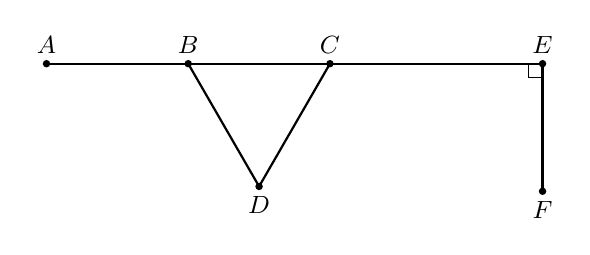
\begin{tikzpicture}[scale=0.9,font=\small]
\draw[thick] (0,0)--(7,0);
\coordinate (A) at (0,0); \coordinate (B) at (2,0); \coordinate (C) at (4,0); \coordinate (E) at (7,0);
\coordinate (D) at (3,-1.732); \coordinate (F) at (7,-1.8);
\draw[thick] (B)--(D)--(C); \draw[thick] (E)--(F);
\draw (6.8,0)--(6.8,-0.2)--(7,-0.2);
\foreach \p/\q in {A/above,B/above,C/above,E/above,D/below,F/below} \fill (\p) circle(1.5pt) node[\q]{$\p$};
\end{tikzpicture}
\end{LTR}\end{center}
عيّن قيساً لكل من الزوايا الموجهة التالية:
\begin{sq}
\qa $\an{\V{AB}}{\V{BD}}$.
\qb $\an{\V{CE}}{\V{CD}}$.
\qc $\an{\V{CE}}{\V{EF}}$.
\qd $\an{\V{BD}}{\V{EF}}$.
\end{sq}
\end{tamrin}
\begin{hal}
من الشكل: $D$ تحت المستقيم $(AE)$ ، ومنه الزوايا الداخلية للمثلث $BCD$: $\an{\V{BC}}{\V{BD}}=-\dfrac{\pi}{3}$ ، $\an{\V{CD}}{\V{CB}}=-\dfrac{\pi}{3}$.\par
والأشعة $\V{AB}$ ، $\V{BC}$ ، $\V{CE}$ لها نفس الاتجاه.
\pa $\an{\V{AB}}{\V{BD}}=\an{\V{BC}}{\V{BD}}=\bx{-\dfrac{\pi}{3}}$ \ (لأن $\V{AB}$ و $\V{BC}$ لهما نفس الاتجاه).
\pb $\an{\V{CE}}{\V{CD}}=\an{-\V{CB}}{\V{CD}}=\an{\V{CB}}{\V{CD}}+\pi=\dfrac{\pi}{3}+\pi=\dfrac{4\pi}{3}$ ، أي القيس الرئيسي \bx{-\dfrac{2\pi}{3}}.
\pc $\an{\V{CE}}{\V{EF}}=\an{\V{EC}}{\V{EF}}+\pi$ (لأن $\V{CE}=-\V{EC}$) $=\dfrac{\pi}{2}+\pi=\dfrac{3\pi}{2}$ ، والقيس الرئيسي \bx{-\dfrac{\pi}{2}}.
\pd بعلاقة شال: $\an{\V{BD}}{\V{EF}}=\an{\V{BD}}{\V{CE}}+\an{\V{CE}}{\V{EF}}$.\par
$\an{\V{BD}}{\V{CE}}=\an{\V{BD}}{\V{BC}}=-\an{\V{BC}}{\V{BD}}=\dfrac{\pi}{3}$ ، إذن $\an{\V{BD}}{\V{EF}}=\dfrac{\pi}{3}-\dfrac{\pi}{2}=\bx{-\dfrac{\pi}{6}}$.
\end{hal}
\begin{molahada}
أقياس هذا التمرين تتعلق باتجاه الشكل: إذا كانت $D$ و $F$ فوق المستقيم $(AE)$ تتغير الإشارات (نجد عندئذ $\dfrac{\pi}{3}$ ، $\dfrac{2\pi}{3}$ ، $\dfrac{\pi}{2}$ ، $\dfrac{\pi}{6}$) ، لذلك يجب دائماً قراءة اتجاه الدوران على الشكل.
\end{molahada}

% ------------------------------------------------- 4
\begin{tamrin}{زاوية محيطية: مثلث ودائرة}
$ABC$ مثلث متقايس الأضلاع ، و $ACD$ مثلث قائم في $A$ حيث $\an{\V{DC}}{\V{DA}}=-\dfrac{\pi}{6}$ ، و $\an{\V{AC}}{\V{AB}}$ زاوية قيسها $-\dfrac{\pi}{3}$. \ $E$ نقطة من الدائرة $(C)$ المحيطة بالمثلث $ADC$ ذات المركز $O$ (منتصف $[DC]$).
\begin{center}\begin{LTR}
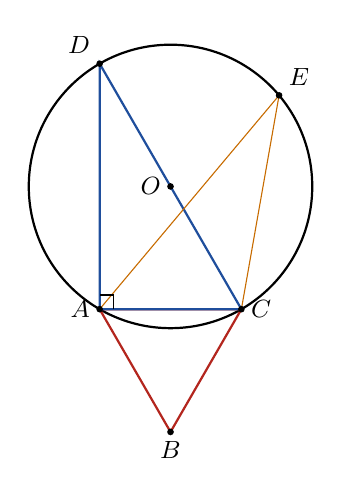
\begin{tikzpicture}[scale=0.6,font=\small]
\coordinate (A) at (0,0); \coordinate (C) at (3,0); \coordinate (D) at (0,5.196); \coordinate (B) at (1.5,-2.598);
\coordinate (O) at (1.5,2.598); \coordinate (E) at (3.798,4.526);
\draw[thick] (O) circle(3);
\draw[cThm,thick] (A)--(B)--(C)--cycle; \draw[cDef,thick] (A)--(C)--(D)--cycle;
\draw[cEx] (E)--(A); \draw[cEx] (E)--(C);
\draw (0.3,0)--(0.3,0.3)--(0,0.3);
\foreach \p/\q in {A/left,B/below,C/right,D/above left,E/above right,O/left} \fill (\p) circle(2pt) node[\q]{$\p$};
\end{tikzpicture}
\end{LTR}\end{center}
\begin{enumerate}
\item عيّن القيس الرئيسي لكل من الزاويتين: $\an{\V{CA}}{\V{CB}}$ و $\an{\V{CD}}{-2\V{CA}}$.
\item عيّن قيساً رئيسياً للزاوية $\an{\V{EA}}{\V{EC}}$ ، مستنتجاً قيساً لـ $\an{\V{OA}}{\V{OC}}$.
\item استنتج نوع المثلث $ACO$.
\item بيّن أن العدد $\dfrac{2018\pi}{6}$ هو قيس للزاوية $\an{\V{OA}}{\V{OC}}$.
\end{enumerate}
\end{tamrin}
\begin{hal}
\textbf{1.} المثلث $ABC$ متقايس الأضلاع و $\an{\V{AC}}{\V{AB}}=-\dfrac{\pi}{3}$ ، فهو مثلث مباشر $ABC$ حيث $\an{\V{CA}}{\V{CB}}=\bx{\dfrac{\pi}{3}}$ (نفس اتجاه الدوران في كل الرؤوس).\par
في المثلث $ACD$ (مجموع الزوايا الموجهة لمثلث يساوي $\pi$):
\[\an{\V{CD}}{\V{CA}}+\an{\V{AC}}{\V{AD}}+\an{\V{DA}}{\V{DC}}=\pi\ \Rightarrow\ \an{\V{CD}}{\V{CA}}+\frac{\pi}{2}+\frac{\pi}{6}=\pi\ \Rightarrow\ \an{\V{CD}}{\V{CA}}=\frac{\pi}{3}.\]
$\an{\V{CD}}{-2\V{CA}}=\an{\V{CD}}{\V{CA}}+\pi=\dfrac{\pi}{3}+\pi=\dfrac{4\pi}{3}$ ، والقيس الرئيسي \bx{-\dfrac{2\pi}{3}}.

\QQ{2} الزاويتان المحيطيتان $\an{\V{EA}}{\V{EC}}$ و $\an{\V{DA}}{\V{DC}}$ تحصران نفس القوس ، إذن: $\an{\V{EA}}{\V{EC}}=\an{\V{DA}}{\V{DC}}=\bx{\dfrac{\pi}{6}}$.\par
حسب مبرهنة الزاوية المحيطية: $\an{\V{OA}}{\V{OC}}=2\an{\V{EA}}{\V{EC}}=2\times\dfrac{\pi}{6}=\bx{\dfrac{\pi}{3}}$.

\QQ{3} $OA=OC$ (نصفا قطر) والزاوية بينهما $\dfrac{\pi}{3}$ ، إذن المثلث $ACO$ \textbf{متقايس الأضلاع}.

\QQ{4} $\dfrac{2018\pi}{6}=\dfrac{2016\pi+2\pi}{6}=336\pi+\dfrac{\pi}{3}=168(2\pi)+\dfrac{\pi}{3}$.\par
الفرق بين $\dfrac{2018\pi}{6}$ و $\dfrac{\pi}{3}$ هو $168\times2\pi$ ، إذن $\dfrac{2018\pi}{6}$ \textbf{قيس للزاوية} $\an{\V{OA}}{\V{OC}}$.
\end{hal}
\begin{molahada}
في الحل المتداول لهذا التمرين: (1) كُتب القيس الرئيسي لـ $\an{\V{CD}}{-2\V{CA}}$ هو $\dfrac{4\pi}{3}$ ، والصحيح $-\dfrac{2\pi}{3}$ لأن $\dfrac{4\pi}{3}\notin\,]-\pi;\pi]$. \ (2) في نص السؤال 4 كُتب $\an{\V{OC}}{\V{OA}}$ ، والصحيح $\an{\V{OA}}{\V{OC}}$ لأن قيسها الرئيسي $\dfrac{\pi}{3}$ أما $\an{\V{OC}}{\V{OA}}$ فقيسها الرئيسي $-\dfrac{\pi}{3}$.
\end{molahada}

% ------------------------------------------------- 5
\begin{tamrin}{مربع ومثلث متساوي الساقين ودائرة}
في المستوي الموجه ، $ABCD$ مربع مباشر ، و $(C)$ الدائرة التي مركزها $D$ ونصف قطرها $DC$. \ $E$ نقطة من $(C)$ حيث $ACE$ مثلث متساوي الساقين رأسه $E$ (أنظر الشكل).
\RL{0.55}{%
\begin{enumerate}
\item عيّن قيساً لكل من الزاويتين الموجهتين $\an{\V{DA}}{\V{DC}}$ و $\an{\V{EA}}{\V{EC}}$.
\item بيّن أن المثلثين $EDC$ و $EDA$ متقايسان.
\item عيّن قيساً لكل من $\an{\V{DC}}{\V{DE}}$ و $\an{\V{DE}}{\V{DA}}$.
\item بيّن أن: $\an{\V{DB}}{\V{DC}}+\an{\V{DC}}{\V{DE}}=\pi$.
\item ماذا يمكنك القول عن النقط $E$ ، $D$ و $B$؟
\end{enumerate}}
{0.4}{%
\begin{center}\begin{LTR}
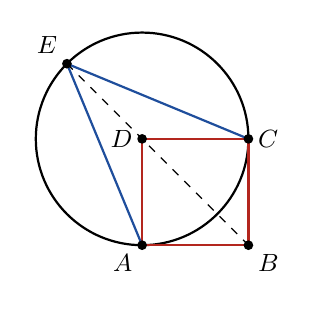
\begin{tikzpicture}[scale=1.35,font=\small]
\coordinate (A) at (0,0); \coordinate (B) at (1,0); \coordinate (C) at (1,1); \coordinate (D) at (0,1);
\coordinate (E) at (-0.7071,1.7071);
\draw[thick] (D) circle(1);
\draw[cThm,thick] (A)--(B)--(C)--(D)--cycle;
\draw[cDef,thick] (E)--(A); \draw[cDef,thick] (E)--(C);
\draw[dashed] (E)--(B);
\foreach \p/\q in {A/below left,B/below right,C/right,D/left,E/above left} \fill (\p) circle(1.3pt) node[\q]{$\p$};
\end{tikzpicture}
\end{LTR}\end{center}}
\end{tamrin}
\begin{hal}
\textbf{1.} المربع مباشر: $\an{\V{DA}}{\V{DC}}=\bx{\dfrac{\pi}{2}}$ (من الشعاع النازل إلى الشعاع الأفقي نحو اليمين: ربع دورة في الاتجاه المباشر).\par
$A$ ، $C$ و $E$ على الدائرة $(C)$ التي مركزها $D$: \ $\an{\V{EA}}{\V{EC}}=\dfrac12\an{\V{DA}}{\V{DC}}=\bx{\dfrac{\pi}{4}}$ (زاوية محيطية).

\QQ{2} $DA=DC$ (ضلعا المربع) ، $EA=EC$ (المثلث متساوي الساقين) ، $DE$ ضلع مشترك: المثلثان $EDC$ و $EDA$ \textbf{متقايسان} (الأضلاع الثلاثة).

\QQ{3} من التقايس: الزاويتان الهندسيتان $\widehat{EDC}$ و $\widehat{EDA}$ متقايستان ، ومجموعهما مع $\widehat{ADC}=\dfrac{\pi}{2}$ يساوي $2\pi$ ، إذن كل منهما $\dfrac{3\pi}{4}$.\par
مع مراعاة الاتجاه: \ $\an{\V{DC}}{\V{DE}}=\bx{\dfrac{3\pi}{4}}$ \ و \ $\an{\V{DE}}{\V{DA}}=\bx{\dfrac{3\pi}{4}}$.\par
(تحقق بشال: $\an{\V{DC}}{\V{DE}}+\an{\V{DE}}{\V{DA}}+\an{\V{DA}}{\V{DC}}=\dfrac{3\pi}{4}+\dfrac{3\pi}{4}+\dfrac{\pi}{2}=2\pi$ \ok.)

\QQ{4} $[DB]$ قطر المربع ، فـ $\an{\V{DB}}{\V{DC}}=\dfrac{\pi}{4}$ ، ومنه: $\an{\V{DB}}{\V{DC}}+\an{\V{DC}}{\V{DE}}=\dfrac{\pi}{4}+\dfrac{3\pi}{4}=\bx{\pi}$.

\QQ{5} بشال: $\an{\V{DB}}{\V{DE}}=\pi$ ، فالشعاعان $\V{DB}$ و $\V{DE}$ متعاكسان: \bx{E\ ،\ D\ ،\ B\ \text{\ar{على استقامة واحدة}}}.
\end{hal}

% ------------------------------------------------- 6
\begin{tamrin}{مثلث قائم ومتساوي الساقين ومنصف زاوية}
في المستوي الموجه ، $ABC$ مثلث قائم في $B$ ومتساوي الساقين حيث $\an{\V{BC}}{\V{BA}}=\dfrac{\pi}{2}$. \ $K$ نقطة تقاطع منصف الزاوية $\widehat{BAC}$ مع الضلع $[BC]$.
\begin{enumerate}
\item عيّن القيس الرئيسي للزوايا الآتية: $\an{\V{AB}}{\V{AK}}$ ، $\an{\V{BC}}{\V{CA}}$ و $\an{\V{KA}}{\V{CB}}$.
\item لتكن $J$ منتصف $[AC]$ و $I$ نقطة تقاطع $(AK)$ و $(BJ)$. حدّد طبيعة المثلث $BIK$.
\end{enumerate}
\end{tamrin}
\begin{hal}
المثلث قائم متساوي الساقين: $\widehat{BAC}=\widehat{BCA}=\dfrac{\pi}{4}$. \ مع $\an{\V{BC}}{\V{BA}}=\dfrac{\pi}{2}$ يكون المثلث $BCA$ مباشراً ، فـ $\an{\V{AB}}{\V{AC}}=\dfrac{\pi}{4}$ و $\an{\V{CA}}{\V{CB}}=\dfrac{\pi}{4}$.
\QQ{1} \begin{itemize}
\item $(AK)$ منصف $\widehat{BAC}$: \ $\an{\V{AB}}{\V{AK}}=\dfrac12\an{\V{AB}}{\V{AC}}=\bx{\dfrac{\pi}{8}}$.
\item $\an{\V{BC}}{\V{CA}}=\an{-\V{CB}}{\V{CA}}=\an{\V{CB}}{\V{CA}}+\pi=-\dfrac{\pi}{4}+\pi=\bx{\dfrac{3\pi}{4}}$.
\item $\an{\V{KA}}{\V{CB}}=\an{\V{KA}}{\V{KB}}$ ($\V{CB}$ و $\V{KB}$ لهما نفس الاتجاه). \ في المثلث $ABK$ القائم في $B$: $\widehat{AKB}=\dfrac{\pi}{2}-\dfrac{\pi}{8}=\dfrac{3\pi}{8}$ ، ومع الاتجاه: $\an{\V{KA}}{\V{CB}}=\bx{\dfrac{3\pi}{8}}$.
\end{itemize}
\QQ{2} $(BJ)$ متوسط في مثلث متساوي الساقين ، فهو أيضاً منصف $\widehat{ABC}$: $\widehat{IBK}=\dfrac{\pi}{4}$.\par
$\widehat{BKI}=\widehat{AKB}=\dfrac{3\pi}{8}$ ، ومنه $\widehat{BIK}=\pi-\dfrac{\pi}{4}-\dfrac{3\pi}{8}=\dfrac{3\pi}{8}$.\par
الزاويتان $\widehat{BKI}$ و $\widehat{BIK}$ متقايستان: المثلث $BIK$ \textbf{متساوي الساقين رأسه $B$} ($BI=BK$).
\end{hal}

% =====================================================================
\section{جيب التمام والجيب والزوايا المرفقة}
% ------------------------------------------------- 7
\begin{tamrin}{القيم المضبوطة}
\begin{enumerate}
\item عيّن القيمة المضبوطة لـ $\cos x$ و $\sin x$ في كل حالة: \ $x=\dfrac{\pi}{6}$ ؛ \ $x=\dfrac{2\pi}{3}$ ؛ \ $x=-\dfrac{\pi}{4}$ ؛ \ $x=\dfrac{4\pi}{3}$.
\item $\alpha$ قيس الزاوية الموجهة التي قيسها $\dfrac{2025\pi}{4}$.
\begin{sq}
\qa عيّن القيس الرئيسي لها ، ثم القيمة المضبوطة لكل من $\cos\alpha$ و $\sin\alpha$.
\qb استنتج القيمة المضبوطة لكل من $\cos(\pi-\alpha)$ و $\sin\Big(\dfrac{\pi}{2}+\alpha\Big)$.
\end{sq}
\item احسب: \ $\cos\dfrac{193\pi}{3}$ ، \ $\sin\dfrac{193\pi}{3}$ ، \ $\cos\Big(-\dfrac{\pi}{6}\Big)$ ، \ $\sin\Big(-\dfrac{\pi}{6}\Big)$ ، \ $\sin\dfrac{55\pi}{4}$ ، \ $\cos\dfrac{17\pi}{6}$.
\end{enumerate}
\end{tamrin}
\begin{hal}
\textbf{1.} \begin{itemize}
\item $\cos\dfrac{\pi}{6}=\dfrac{\sqrt3}{2}$ ، $\sin\dfrac{\pi}{6}=\dfrac12$.
\item $\dfrac{2\pi}{3}=\pi-\dfrac{\pi}{3}$: \ $\cos\dfrac{2\pi}{3}=-\cos\dfrac{\pi}{3}=-\dfrac12$ ، \ $\sin\dfrac{2\pi}{3}=\sin\dfrac{\pi}{3}=\dfrac{\sqrt3}{2}$.
\item $\cos\Big(-\dfrac{\pi}{4}\Big)=\cos\dfrac{\pi}{4}=\dfrac{\sqrt2}{2}$ ، \ $\sin\Big(-\dfrac{\pi}{4}\Big)=-\sin\dfrac{\pi}{4}=-\dfrac{\sqrt2}{2}$.
\item $\dfrac{4\pi}{3}=\pi+\dfrac{\pi}{3}$: \ $\cos\dfrac{4\pi}{3}=-\dfrac12$ ، \ $\sin\dfrac{4\pi}{3}=-\dfrac{\sqrt3}{2}$.
\end{itemize}
\QQ{2} \pa $\dfrac{2025\pi}{4}=506\pi+\dfrac{\pi}{4}$: القيس الرئيسي \bx{\dfrac{\pi}{4}} ، و $\cos\alpha=\sin\alpha=\bx{\dfrac{\sqrt2}{2}}$.
\pb $\cos(\pi-\alpha)=-\cos\alpha=\bx{-\dfrac{\sqrt2}{2}}$ \ ؛ \ $\sin\Big(\dfrac{\pi}{2}+\alpha\Big)=\cos\alpha=\bx{\dfrac{\sqrt2}{2}}$.
\QQ{3} \begin{itemize}
\item $\dfrac{193\pi}{3}=64\pi+\dfrac{\pi}{3}$: \ $\cos\dfrac{193\pi}{3}=\cos\dfrac{\pi}{3}=\bx{\dfrac12}$ ، \ $\sin\dfrac{193\pi}{3}=\sin\dfrac{\pi}{3}=\bx{\dfrac{\sqrt3}{2}}$.
\item $\cos\Big(-\dfrac{\pi}{6}\Big)=\bx{\dfrac{\sqrt3}{2}}$ ، \ $\sin\Big(-\dfrac{\pi}{6}\Big)=\bx{-\dfrac12}$.
\item $\dfrac{55\pi}{4}=14\pi-\dfrac{\pi}{4}$: \ $\sin\dfrac{55\pi}{4}=\sin\Big(-\dfrac{\pi}{4}\Big)=\bx{-\dfrac{\sqrt2}{2}}$.
\item $\dfrac{17\pi}{6}=2\pi+\pi-\dfrac{\pi}{6}$: \ $\cos\dfrac{17\pi}{6}=\cos\Big(\pi-\dfrac{\pi}{6}\Big)=-\cos\dfrac{\pi}{6}=\bx{-\dfrac{\sqrt3}{2}}$.
\end{itemize}
\end{hal}

% ------------------------------------------------- 8
\begin{tamrin}{تبسيط عبارات وإثبات مساويات}
\begin{enumerate}
\item بسّط العبارات التالية:
\begin{sq}
\qa $A=\sin\Big(\dfrac{\pi}{2}-x\Big)+\cos(\pi-x)+\cos(\pi+x)$.
\qb $B=\cos(\pi-x)-\cos x+\sin(\pi+x)+\cos\Big(\dfrac{\pi}{2}-x\Big)$.
\qc $C(x)=\cos(2023\pi+x)+\sin\Big(\dfrac{21\pi}{2}-x\Big)+\cos(1988\pi-x)$.
\end{sq}
\item أثبت أنه من أجل كل عدد حقيقي $x$:
\begin{sq}
\qa $\sin\Big(\dfrac{5\pi}{2}+x\Big)-2\cos\Big(\dfrac{21\pi}{2}-x\Big)-3\sin(x-3\pi)+\sin\Big(\dfrac{3\pi}{2}+x\Big)=\sin x$.
\qb $\sin(x+7\pi)-2\sin\Big(x-\dfrac{\pi}{2}\Big)=2\sin\Big(\dfrac{13\pi}{2}-x\Big)-\cos\Big(x+\dfrac{7\pi}{2}\Big)$.
\end{sq}
\end{enumerate}
\end{tamrin}
\begin{hal}
\textbf{1.} \pa $A=\cos x-\cos x-\cos x=\bx{-\cos x}$.
\pb $B=-\cos x-\cos x-\sin x+\sin x=\bx{-2\cos x}$.
\pc $\cos(2023\pi+x)=\cos(2022\pi+\pi+x)=\cos(\pi+x)=-\cos x$ ؛\par
$\sin\Big(\dfrac{21\pi}{2}-x\Big)=\sin\Big(10\pi+\dfrac{\pi}{2}-x\Big)=\sin\Big(\dfrac{\pi}{2}-x\Big)=\cos x$ ؛ \ $\cos(1988\pi-x)=\cos(-x)=\cos x$.\par
إذن $C(x)=-\cos x+\cos x+\cos x=\bx{\cos x}$.

\QQ{2} \pa نبسط كل حد:
\begin{itemize}
\item $\sin\Big(\dfrac{5\pi}{2}+x\Big)=\sin\Big(2\pi+\dfrac{\pi}{2}+x\Big)=\sin\Big(\dfrac{\pi}{2}+x\Big)=\cos x$.
\item $\cos\Big(\dfrac{21\pi}{2}-x\Big)=\cos\Big(\dfrac{\pi}{2}-x\Big)=\sin x$ ، ومنه $-2\cos\Big(\dfrac{21\pi}{2}-x\Big)=-2\sin x$.
\item $\sin(x-3\pi)=\sin(x-\pi-2\pi)=\sin(x-\pi)=-\sin(\pi-x)=-\sin x$ ، ومنه $-3\sin(x-3\pi)=3\sin x$.
\item $\sin\Big(\dfrac{3\pi}{2}+x\Big)=\sin\Big(\pi+\dfrac{\pi}{2}+x\Big)=-\sin\Big(\dfrac{\pi}{2}+x\Big)=-\cos x$.
\end{itemize}
المجموع: $\cos x-2\sin x+3\sin x-\cos x=\sin x$ \ok.
\pb \textbf{الطرف الأيسر:} $\sin(x+7\pi)=\sin(x+\pi)=-\sin x$ ؛ \ $\sin\Big(x-\dfrac{\pi}{2}\Big)=-\sin\Big(\dfrac{\pi}{2}-x\Big)=-\cos x$. \ إذن الطرف الأيسر $=-\sin x+2\cos x$.\par
\textbf{الطرف الأيمن:} $\sin\Big(\dfrac{13\pi}{2}-x\Big)=\sin\Big(\dfrac{\pi}{2}-x\Big)=\cos x$ ؛ \ $\cos\Big(x+\dfrac{7\pi}{2}\Big)=\cos\Big(x+\dfrac{3\pi}{2}\Big)=\cos\Big(\pi+\dfrac{\pi}{2}+x\Big)=-\cos\Big(\dfrac{\pi}{2}+x\Big)=\sin x$.\par
إذن الطرف الأيمن $=2\cos x-\sin x$: الطرفان متساويان \ok.
\end{hal}

% ------------------------------------------------- 9
\begin{tamrin}{من الظل إلى الجيب وجيب التمام (تمرين نموذجي)}
$x$ عدد حقيقي من المجال $\Big]\pi;\dfrac{3\pi}{2}\Big[$ حيث: $\dfrac{\sin x}{\cos x}=\dfrac{\sqrt5}{2}$.
\begin{enumerate}
\item احسب القيمة المضبوطة لكل من $\cos x$ و $\sin x$.
\item استنتج: $\sin(\pi+x)$ ، $\sin(\pi-x)$ ، $\cos(\pi+x)$ و $\cos(\pi-x)$.
\end{enumerate}
\end{tamrin}
\begin{hal}
\textbf{1.} $\sin x=\dfrac{\sqrt5}{2}\cos x$. نعوّض في $\cos^2x+\sin^2x=1$: $\cos^2x+\dfrac54\cos^2x=1$ ، أي $\dfrac94\cos^2x=1$ ، ومنه $\cos^2x=\dfrac49$.\par
$x\in\Big]\pi;\dfrac{3\pi}{2}\Big[$ (الربع الثالث): $\cos x<0$ و $\sin x<0$ ، إذن \bx{\cos x=-\dfrac23} و $\sin x=\dfrac{\sqrt5}{2}\times\Big(-\dfrac23\Big)=\bx{-\dfrac{\sqrt5}{3}}$.
\QQ{2} $\sin(\pi+x)=-\sin x=\dfrac{\sqrt5}{3}$ ؛ \ $\sin(\pi-x)=\sin x=-\dfrac{\sqrt5}{3}$ ؛ \ $\cos(\pi+x)=\cos(\pi-x)=-\cos x=\dfrac23$.
\end{hal}

% =====================================================================
\section{المعادلات والمتراجحات المثلثية}
% ------------------------------------------------- 10
\begin{tamrin}{معادلات أساسية}
\begin{enumerate}
\item حل في $\R$ المعادلات التالية ، ثم مثّل صور الحلول على الدائرة المثلثية:
\begin{sq}
\qa $2\cos x-\sqrt3=0$.
\qb $2\sin x-1=0$.
\qc $\cos x-1=0$.
\qd $\sin x=-1$.
\end{sq}
\item حل في المجال $I=[-\pi;\pi]$ المعادلة: $\sqrt2\cos x-1=0$.
\item حل في المجال $[0;2\pi]$ المعادلة: $2\sin x-\sqrt3=0$.
\end{enumerate}
\end{tamrin}
\begin{hal}
\textbf{1.} \pa $\cos x=\dfrac{\sqrt3}{2}=\cos\dfrac{\pi}{6}$: \ \bx{S=\Big\{\dfrac{\pi}{6}+2k\pi\,;\,-\dfrac{\pi}{6}+2k\pi\,/\,k\in\Z\Big\}}.
\pb $\sin x=\dfrac12=\sin\dfrac{\pi}{6}$: \ $x=\dfrac{\pi}{6}+2k\pi$ أو $x=\pi-\dfrac{\pi}{6}+2k\pi$: \ \bx{S=\Big\{\dfrac{\pi}{6}+2k\pi\,;\,\dfrac{5\pi}{6}+2k\pi\Big\}}.
\pc $\cos x=1$: \ \bx{S=\{2k\pi\,/\,k\in\Z\}}.
\pd $\sin x=-1$: \ \bx{S=\Big\{-\dfrac{\pi}{2}+2k\pi\,/\,k\in\Z\Big\}}.
\begin{center}\begin{LTR}
\begin{tikzpicture}[scale=1.3,font=\scriptsize]
\begin{scope}\TrigCircle
\fill[cThm] (30:1) circle(1.5pt) node[right]{$\frac{\pi}{6}$}; \fill[cThm] (-30:1) circle(1.5pt) node[right]{$-\frac{\pi}{6}$};
\node at (0,-1.6){(أ)};\end{scope}
\begin{scope}[xshift=3.2cm]\TrigCircle
\fill[cThm] (30:1) circle(1.5pt) node[right]{$\frac{\pi}{6}$}; \fill[cThm] (150:1) circle(1.5pt) node[left]{$\frac{5\pi}{6}$};
\node at (0,-1.6){(ب)};\end{scope}
\begin{scope}[xshift=6.4cm]\TrigCircle
\fill[cThm] (0:1) circle(1.5pt) node[above right]{$0$};
\node at (0,-1.6){(جـ)};\end{scope}
\begin{scope}[xshift=9.6cm]\TrigCircle
\fill[cThm] (-90:1) circle(1.5pt) node[below right]{$-\frac{\pi}{2}$};
\node at (0,-1.6){(د)};\end{scope}
\end{tikzpicture}
\end{LTR}\end{center}
\QQ{2} $\cos x=\dfrac{\sqrt2}{2}=\cos\dfrac{\pi}{4}$: $x=\pm\dfrac{\pi}{4}+2k\pi$. \ في $[-\pi;\pi]$ (نأخذ $k=0$): \bx{S=\Big\{-\dfrac{\pi}{4};\dfrac{\pi}{4}\Big\}}.
\QQ{3} $\sin x=\dfrac{\sqrt3}{2}=\sin\dfrac{\pi}{3}$: $x=\dfrac{\pi}{3}+2k\pi$ أو $x=\dfrac{2\pi}{3}+2k\pi$. \ في $[0;2\pi]$: \bx{S=\Big\{\dfrac{\pi}{3};\dfrac{2\pi}{3}\Big\}}.
\end{hal}

% ------------------------------------------------- 11
\begin{tamrin}{معادلات تؤول إلى معادلات أساسية}
\begin{enumerate}
\item حل في المجال $]-\pi;2\pi]$ المعادلة: $\cos x\big(\sqrt2\sin x-1\big)=0$.
\item حل في $\R$ المعادلتين: \ $\sin^2x-\sin x-6=0$ \ و \ $2\cos^2x-3\cos x-2=0$.
\item حل في $\R$ المعادلة: $\sin x+\cos x=1$. \ (إرشاد: ربّع الطرفين ثم تحقق.)
\item حل في المجال $]-\pi;\pi]$ المعادلة: $\sqrt2\cos(3x)+1=0$.
\item حل في $[-\pi;\pi]$ المعادلة: $\cos x\sin^2x+\cos x\sin x-2\cos x=0$.
\end{enumerate}
\end{tamrin}
\begin{hal}
\textbf{1.} جداء معدوم: $\cos x=0$ أو $\sin x=\dfrac{\sqrt2}{2}$.
\begin{itemize}
\item $\cos x=0\iff x=\dfrac{\pi}{2}+k\pi$: في $]-\pi;2\pi]$: $-\dfrac{\pi}{2}$ ، $\dfrac{\pi}{2}$ ، $\dfrac{3\pi}{2}$.
\item $\sin x=\dfrac{\sqrt2}{2}\iff x=\dfrac{\pi}{4}+2k\pi$ أو $x=\dfrac{3\pi}{4}+2k\pi$: في $]-\pi;2\pi]$: $\dfrac{\pi}{4}$ ، $\dfrac{3\pi}{4}$.
\end{itemize}
\bx{S=\Big\{-\dfrac{\pi}{2};\dfrac{\pi}{4};\dfrac{\pi}{2};\dfrac{3\pi}{4};\dfrac{3\pi}{2}\Big\}}.

\QQ{2} \textbf{الأولى:} نضع $X=\sin x$: $X^2-X-6=0$ ، $\Delta=25$ ، $X=3$ أو $X=-2$. \ كلاهما خارج $[-1;1]$: \bx{S=\varnothing}.\par
\textbf{الثانية:} نضع $X=\cos x$: $2X^2-3X-2=0$ ، $\Delta=9+16=25$ ، $X=2$ (مرفوض) أو $X=-\dfrac12$.\par
$\cos x=-\dfrac12=\cos\dfrac{2\pi}{3}$: \ \bx{S=\Big\{\dfrac{2\pi}{3}+2k\pi\,;\,-\dfrac{2\pi}{3}+2k\pi\,/\,k\in\Z\Big\}}.

\QQ{3} إذا كان $\sin x+\cos x=1$ فإن $(\sin x+\cos x)^2=1$ ، أي $1+2\sin x\cos x=1$ ، ومنه $\sin x\cos x=0$:
\begin{itemize}
\item $\sin x=0$: نعوّض: $\cos x=1$ ، أي $x=2k\pi$ \ (الحل $x=\pi+2k\pi$ مرفوض لأن $\cos x=-1$).
\item $\cos x=0$: نعوّض: $\sin x=1$ ، أي $x=\dfrac{\pi}{2}+2k\pi$.
\end{itemize}
\bx{S=\Big\{2k\pi\,;\,\dfrac{\pi}{2}+2k\pi\,/\,k\in\Z\Big\}}.

\QQ{4} $\cos3x=-\dfrac{\sqrt2}{2}=\cos\dfrac{3\pi}{4}$: \ $3x=\pm\dfrac{3\pi}{4}+2k\pi$ ، أي $x=\pm\dfrac{\pi}{4}+\dfrac{2k\pi}{3}$.\par
في $]-\pi;\pi]$: \ من $\dfrac{\pi}{4}+\dfrac{2k\pi}{3}$ ($k=-1;0;1$): $-\dfrac{5\pi}{12}$ ، $\dfrac{\pi}{4}$ ، $\dfrac{11\pi}{12}$ ؛ \ من $-\dfrac{\pi}{4}+\dfrac{2k\pi}{3}$ ($k=-1;0;1$): $-\dfrac{11\pi}{12}$ ، $-\dfrac{\pi}{4}$ ، $\dfrac{5\pi}{12}$.\par
\bx{S=\Big\{-\dfrac{11\pi}{12};-\dfrac{5\pi}{12};-\dfrac{\pi}{4};\dfrac{\pi}{4};\dfrac{5\pi}{12};\dfrac{11\pi}{12}\Big\}}.

\QQ{5} $\cos x\big(\sin^2x+\sin x-2\big)=0$ ، و $\sin^2x+\sin x-2=(\sin x-1)(\sin x+2)$:
\begin{itemize}
\item $\cos x=0$: $x=\pm\dfrac{\pi}{2}$ ؛ \ $\sin x=1$: $x=\dfrac{\pi}{2}$ ؛ \ $\sin x=-2$: مستحيلة.
\end{itemize}
\bx{S=\Big\{-\dfrac{\pi}{2};\dfrac{\pi}{2}\Big\}}.
\end{hal}
\begin{molahada}
في أحد الحلول المتداولة للمعادلة $\sin x+\cos x=1$ كُتب $S=\Big\{k\pi\,;\,\dfrac{\pi}{2}+k\pi\Big\}$ ، وهذا خطأ: مثلاً $x=\pi$ يعطي $\sin\pi+\cos\pi=-1\ne1$. الصحيح $S=\Big\{2k\pi\,;\,\dfrac{\pi}{2}+2k\pi\Big\}$.
\end{molahada}

% ------------------------------------------------- 12
\begin{tamrin}{معادلات من الشكل $\cos u=\cos v$ و $\cos u=\sin v$}
حل في $\R$ المعادلات التالية:
\begin{sq}
\qa $\cos\Big(2x-\dfrac{\pi}{3}\Big)=\dfrac12$.
\qb $\sin\Big(2x+\dfrac{\pi}{4}\Big)=-\dfrac{\sqrt3}{2}$.
\qc $\cos3x=\cos x$.
\qd $\cos x+\sin x=0$.
\qe $\cos\Big(x-\dfrac{\pi}{4}\Big)=\sin\Big(3x+\dfrac{\pi}{3}\Big)$.
\end{sq}
\end{tamrin}
\begin{hal}
\pa $\cos\Big(2x-\dfrac{\pi}{3}\Big)=\cos\dfrac{\pi}{3}$: \ $2x-\dfrac{\pi}{3}=\dfrac{\pi}{3}+2k\pi\iff x=\dfrac{\pi}{3}+k\pi$ ؛ \ أو \ $2x-\dfrac{\pi}{3}=-\dfrac{\pi}{3}+2k\pi\iff x=k\pi$.\par
\bx{S=\Big\{k\pi\,;\,\dfrac{\pi}{3}+k\pi\,/\,k\in\Z\Big\}}.
\pb $\sin\Big(2x+\dfrac{\pi}{4}\Big)=\sin\Big(-\dfrac{\pi}{3}\Big)$:
\begin{itemize}
\item $2x+\dfrac{\pi}{4}=-\dfrac{\pi}{3}+2k\pi\iff2x=-\dfrac{7\pi}{12}+2k\pi\iff x=-\dfrac{7\pi}{24}+k\pi$.
\item $2x+\dfrac{\pi}{4}=\pi+\dfrac{\pi}{3}+2k\pi\iff2x=\dfrac{13\pi}{12}+2k\pi\iff x=\dfrac{13\pi}{24}+k\pi$.
\end{itemize}
\pc $3x=x+2k\pi\iff x=k\pi$ ؛ \ أو $3x=-x+2k\pi\iff x=\dfrac{k\pi}{2}$. \ (الأولى محتواة في الثانية): \bx{S=\Big\{\dfrac{k\pi}{2}\,/\,k\in\Z\Big\}}.
\pd $\cos x=-\sin x=\sin(-x)=\cos\Big(\dfrac{\pi}{2}+x\Big)$:
\begin{itemize}
\item $x=\dfrac{\pi}{2}+x+2k\pi$: مستحيلة.
\item $x=-\dfrac{\pi}{2}-x+2k\pi\iff2x=-\dfrac{\pi}{2}+2k\pi\iff x=-\dfrac{\pi}{4}+k\pi$.
\end{itemize}
\bx{S=\Big\{-\dfrac{\pi}{4}+k\pi\,/\,k\in\Z\Big\}}.
\pe $\sin\Big(3x+\dfrac{\pi}{3}\Big)=\cos\Big(\dfrac{\pi}{2}-3x-\dfrac{\pi}{3}\Big)=\cos\Big(\dfrac{\pi}{6}-3x\Big)$ ، فالمعادلة: $\cos\Big(x-\dfrac{\pi}{4}\Big)=\cos\Big(\dfrac{\pi}{6}-3x\Big)$:
\begin{itemize}
\item $x-\dfrac{\pi}{4}=\dfrac{\pi}{6}-3x+2k\pi\iff4x=\dfrac{5\pi}{12}+2k\pi\iff x=\dfrac{5\pi}{48}+\dfrac{k\pi}{2}$.
\item $x-\dfrac{\pi}{4}=-\dfrac{\pi}{6}+3x+2k\pi\iff-2x=\dfrac{\pi}{12}+2k\pi\iff x=-\dfrac{\pi}{24}+k\pi$.
\end{itemize}
\bx{S=\Big\{\dfrac{5\pi}{48}+\dfrac{k\pi}{2}\,;\,-\dfrac{\pi}{24}+k\pi\,/\,k\in\Z\Big\}}.
\end{hal}
\begin{molahada}
في الحل المتداول للمعادلة (هـ) وُجد $4x=\dfrac{10\pi}{20}+2k\pi$ ، والصحيح $\dfrac{\pi}{6}+\dfrac{\pi}{4}=\dfrac{5\pi}{12}=\dfrac{10\pi}{24}$ ، ومنه $x=\dfrac{5\pi}{48}+\dfrac{k\pi}{2}$.
\end{molahada}

% ------------------------------------------------- 13
\begin{tamrin}{متراجحات مثلثية}
\begin{enumerate}
\item حل في المجال $[-\pi;\pi]$ المتراجحة: $\sqrt2\cos x-1\le0$.
\item حل في المجال $[0;2\pi]$ المتراجحة: $2\sin x-\sqrt3<0$.
\item عيّن مجموعة قيم $x$ من المجال $\Big[-\dfrac{\pi}{2};\dfrac{\pi}{2}\Big]$ حيث: $2\sqrt3\cos x<3$.
\item عيّن مجموعة قيم $x$ من المجال $[0;2\pi[$ حيث: $-\dfrac12\le\cos x\le\dfrac12$.
\item حل في المجال $]-\pi;\pi]$ المتراجحة: $2\cos\Big(\dfrac{\pi}{2}-x\Big)-1\ge0$.
\item حل في المجال $[0;\pi]$ المتراجحة: $2\sin\Big(2x-\dfrac{\pi}{6}\Big)-1\le0$.
\end{enumerate}
\end{tamrin}
\begin{hal}
\textbf{1.} $\cos x\le\dfrac{\sqrt2}{2}$: الحدود $\pm\dfrac{\pi}{4}$ ، و $M$ على يسار المستقيم $x=\dfrac{\sqrt2}{2}$: \ \bx{S=\Big[-\pi;-\dfrac{\pi}{4}\Big]\cup\Big[\dfrac{\pi}{4};\pi\Big]}.
\QQ{2} $\sin x<\dfrac{\sqrt3}{2}$: الحدود $\dfrac{\pi}{3}$ و $\dfrac{2\pi}{3}$ ، و $M$ تحت المستقيم $y=\dfrac{\sqrt3}{2}$: \ \bx{S=\Big[0;\dfrac{\pi}{3}\Big[\cup\Big]\dfrac{2\pi}{3};2\pi\Big]}.
\QQ{3} $\cos x<\dfrac{3}{2\sqrt3}=\dfrac{\sqrt3}{2}$: الحدود $\pm\dfrac{\pi}{6}$: \ \bx{S=\Big[-\dfrac{\pi}{2};-\dfrac{\pi}{6}\Big[\cup\Big]\dfrac{\pi}{6};\dfrac{\pi}{2}\Big]}.
\QQ{4} \begin{itemize}
\item $\cos x\le\dfrac12$ في $[0;2\pi[$: $S_1=\Big[\dfrac{\pi}{3};\dfrac{5\pi}{3}\Big]$.
\item $\cos x\ge-\dfrac12$ في $[0;2\pi[$: $S_2=\Big[0;\dfrac{2\pi}{3}\Big]\cup\Big[\dfrac{4\pi}{3};2\pi\Big[$.
\end{itemize}
$S=S_1\cap S_2=$ \bx{\Big[\dfrac{\pi}{3};\dfrac{2\pi}{3}\Big]\cup\Big[\dfrac{4\pi}{3};\dfrac{5\pi}{3}\Big]}.
\begin{center}\begin{LTR}
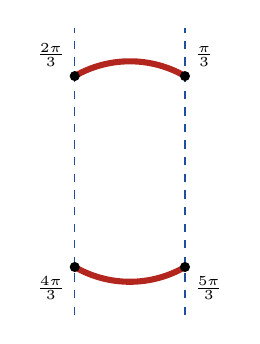
\begin{tikzpicture}[scale=1.4,font=\scriptsize]
\TrigCircle
\draw[cDef,dashed] (0.5,-1.3)--(0.5,1.3); \draw[cDef,dashed] (-0.5,-1.3)--(-0.5,1.3);
\draw[cThm,line width=2.2pt] (60:1) arc(60:120:1); \draw[cThm,line width=2.2pt] (240:1) arc(240:300:1);
\fill (60:1) circle(1.3pt) node[above right]{$\frac{\pi}{3}$}; \fill (120:1) circle(1.3pt) node[above left]{$\frac{2\pi}{3}$};
\fill (240:1) circle(1.3pt) node[below left]{$\frac{4\pi}{3}$}; \fill (300:1) circle(1.3pt) node[below right]{$\frac{5\pi}{3}$};
\end{tikzpicture}
\end{LTR}\end{center}
\QQ{5} $\cos\Big(\dfrac{\pi}{2}-x\Big)=\sin x$ ، فالمتراجحة: $\sin x\ge\dfrac12$: \ \bx{S=\Big[\dfrac{\pi}{6};\dfrac{5\pi}{6}\Big]}.
\QQ{6} نضع $y=2x-\dfrac{\pi}{6}$. إذا كان $x\in[0;\pi]$ فإن $y\in\Big[-\dfrac{\pi}{6};\dfrac{11\pi}{6}\Big]$. \ نحل $\sin y\le\dfrac12$ في هذا المجال:
\[y\in\Big[-\frac{\pi}{6};\frac{\pi}{6}\Big]\cup\Big[\frac{5\pi}{6};\frac{11\pi}{6}\Big].\]
ومنه $x=\dfrac{y}{2}+\dfrac{\pi}{12}$: \ \bx{S=\Big[0;\dfrac{\pi}{6}\Big]\cup\Big[\dfrac{\pi}{2};\pi\Big]}.
\end{hal}

% =====================================================================
\section{الاختيار من متعدد وصحيح أم خطأ}
% ------------------------------------------------- 14
\begin{tamrin}{اختيار من متعدد}
عيّن الاقتراح الصحيح الوحيد في كل حالة مع التعليل:
\begin{enumerate}
\item القيس الرئيسي للزاوية التي قيسها $\dfrac{-39\pi}{4}$ هو:
\ABC{$-\dfrac{\pi}{4}$}{$\dfrac{\pi}{4}$}{$\dfrac{3\pi}{4}$}
\item إذا كان $\an{\vu}{\vv}=\dfrac{\pi}{6}$ فإن $\an{-\vv}{2\vu}$ يساوي:
\ABC{$\dfrac{5\pi}{6}$}{$-\dfrac{\pi}{6}$}{$\dfrac{7\pi}{6}$}
\item $\cos\Big(\dfrac{\pi}{2}+x\Big)+\sin(\pi-x)$ يساوي:
\ABC{$0$}{$2\sin x$}{$-2\sin x$}
\item حلول المعادلة $\cos x=\cos\dfrac{\pi}{5}$ في $]-\pi;\pi]$:
\ABC{$\Big\{\dfrac{\pi}{5}\Big\}$}{$\Big\{-\dfrac{\pi}{5};\dfrac{\pi}{5}\Big\}$}{$\Big\{\dfrac{\pi}{5};\dfrac{4\pi}{5}\Big\}$}
\item عدد حلول المعادلة $\sin x=\dfrac{3}{2}$ في $\R$:
\ABC{$0$}{$2$}{\ar{عدد لا نهائي}}
\item إذا كانت $A$ ، $B$ ، $M$ نقطاً من دائرة مركزها $O$ و $\an{\V{OA}}{\V{OB}}=\dfrac{2\pi}{3}$ فإن $\an{\V{MA}}{\V{MB}}$ يساوي:
\ABC{$\dfrac{2\pi}{3}$}{$\dfrac{4\pi}{3}$}{$\dfrac{\pi}{3}$}
\end{enumerate}
\end{tamrin}
\begin{hal}
\textbf{1.} (ب): $-\dfrac{39\pi}{4}=-10\pi+\dfrac{\pi}{4}$: \bx{\dfrac{\pi}{4}}.
\QQ{2} (أ): $\an{-\vv}{2\vu}=\an{\vv}{\vu}+\pi$ ($-1$ و $2$ مختلفان في الإشارة) $=-\dfrac{\pi}{6}+\pi=\bx{\dfrac{5\pi}{6}}$.
\QQ{3} (أ): $-\sin x+\sin x=\bx{0}$.
\QQ{4} (ب): $x=\pm\dfrac{\pi}{5}+2k\pi$ ، وفي $]-\pi;\pi]$: \bx{\Big\{-\dfrac{\pi}{5};\dfrac{\pi}{5}\Big\}}.
\QQ{5} (أ): $\dfrac32>1$ و $\sin x\le1$: \bx{0} حلول.
\QQ{6} (جـ): الزاوية المحيطية: $\an{\V{MA}}{\V{MB}}=\dfrac12\an{\V{OA}}{\V{OB}}=\bx{\dfrac{\pi}{3}}$ \ (بترديد $\pi$).
\end{hal}

% ------------------------------------------------- 15
\begin{tamrin}{صحيح أم خطأ}
أجب بصحيح أو خطأ مع التبرير:
\begin{enumerate}
\item العددان $\dfrac{17\pi}{4}$ و $-\dfrac{7\pi}{4}$ قيسان لنفس الزاوية الموجهة.
\item من أجل كل عدد حقيقي $x$: $\sin(\pi+x)+\sin(-x)=0$.
\item القيس الرئيسي للزاوية $\an{\vu}{-\vu}$ هو $-\pi$.
\item إذا كان $\cos a=\cos b$ فإن $a=b$.
\item مجموعة حلول المتراجحة $\cos x>1$ في $\R$ هي المجموعة الخالية.
\end{enumerate}
\end{tamrin}
\begin{hal}
\textbf{1. صحيح:} $\dfrac{17\pi}{4}+\dfrac{7\pi}{4}=\dfrac{24\pi}{4}=6\pi=3\times2\pi$.
\QQ{2} \textbf{خطأ:} $\sin(\pi+x)+\sin(-x)=-\sin x-\sin x=-2\sin x$ ، وهو لا ينعدم دائماً (مثلاً $x=\dfrac{\pi}{2}$).
\QQ{3} \textbf{خطأ:} القيس الرئيسي ينتمي إلى $]-\pi;\pi]$ و $-\pi\notin\,]-\pi;\pi]$ ؛ القيس الرئيسي هو $\pi$.
\QQ{4} \textbf{خطأ:} مثال مضاد: $\cos\dfrac{\pi}{3}=\cos\Big(-\dfrac{\pi}{3}\Big)$ و $\dfrac{\pi}{3}\ne-\dfrac{\pi}{3}$.
\QQ{5} \textbf{صحيح:} من أجل كل $x$: $\cos x\le1$.
\end{hal}

\end{document}
